\documentclass[14pt,aspectratio=1610]{beamer}

\usepackage[brazil]{babel}
\usepackage[utf8]{inputenc}
%\UseRawInputEncoding
\usepackage[T1]{fontenc}
%\usepackage{Sweave}
\usepackage{animate}
\usepackage{amsbsy}
\usepackage{amsfonts}
\usepackage{amsmath}
\usepackage{amssymb}
\usepackage{amsthm}
\usepackage[toc,page,title,titletoc]{appendix}
%\usepackage[fixlanguage]{babelbib}
%\usepackage[pdftex]{color}
\usepackage{dsfont}
\usepackage{esvect}
\usepackage[labelfont=bf]{caption}
\usepackage{subcaption}
\usepackage{float}
\usepackage{verbatim}
\usepackage[Glenn]{fncychap}%Sonny %Conny %Lenny %Glenn %Renje %Bjarne %Bjornstrup
%\usepackage{geometry, calc, color, setspace}%
%\geometry{a4paper, headsep=1.0cm, footskip=1cm, lmargin=3cm, rmargin=2cm, tmargin=3cm, bmargin=2cm}
\usepackage{graphicx}
\usepackage{indentfirst}%Para indentar os parágrafos automáticamente
\usepackage{lipsum}
\usepackage{longtable}
\usepackage{mathtools}
\usepackage{listings}%Inserir codigo do R no latex
%\usepackage{slashbox}
\usepackage{multirow}
\usepackage{multicol}
\usepackage{csquotes}
\usepackage[citestyle=authoryear,maxcitenames=2,terseinits=true,natbib=true, style=abnt, maxbibnames=99]{biblatex}
\addbibresource{Referencias/Referencias.bib}
\usepackage[figuresright]{rotating}
\usepackage{spalign}
%\usepackage{pgfpages}
\usepackage{pgfplots}
\pgfplotsset{compat=1.18}
\usepackage{tikz}
\usepackage{color, colortbl}
\usepackage{ragged2e}%para justificar o texto dentro de algum ambiente
\definecolor{Gray}{gray}{0.9}
\definecolor{LightCyan}{rgb}{0.88,1,1}
\definecolor{Lightblue}{RGB}{50, 149, 168}
%\usepackage{grffile}

\usepackage[all]{xy}



\usetheme{Madrid}
\usecolortheme[RGB={193,0,0}]{structure}

%\setbeamertemplate{footline}[frame number]
%\setbeamertemplate{footline}[text line]{%
%  \parbox{\linewidth}{\vspace*{-8pt}\hfill\date{}\hfill\insertshortauthor\hfill\insertpagenumber}}
\beamertemplatenavigationsymbolsempty
\renewcommand{\vec}[1]{\mbox{\boldmath$#1$}}
\newtheorem{Teorema}{Teorema}
\newtheorem{Proposicao}{Proposição}
\newtheorem{Definicao}{Definição}
\newtheorem{Corolario}{Corolário}
\newtheorem{Demonstracao}{Demonstração}
\newcommand{\bx}{\ensuremath{\bar{x}}}
\newcommand{\Ho}{\ensuremath{H_{0}}}
\newcommand{\Hi}{\ensuremath{H_{1}}}
\everymath{\displaystyle}

\apptocmd{\frame}{}{\justifying}{} % Allow optional arguments after frame.

\title{Estatística I}
\author{Prof. Fernando de Souza Bastos \texorpdfstring{\\ fernando.bastos@ufv.br}{}}
\institute{Departamento de Estatística \texorpdfstring{\\ Universidade Federal de Viçosa}{}\texorpdfstring{\\ Campus UFV - Viçosa}{}}
\date{}
\newcommand\mytext{Aula 19}
\newcommand\mytextt{Fernando de Souza Bastos}
\newcommand\mytexttt{\url{https://ufvest.github.io/}}

\makeatletter
\setbeamertemplate{footline}
{
  \leavevmode%
  \hbox{%
  \begin{beamercolorbox}[wd=.3\paperwidth,ht=2.25ex,dp=1ex,center]{author in head/foot}%
    \usebeamerfont{author in head/foot}\mytext
  \end{beamercolorbox}%
  \begin{beamercolorbox}[wd=.3\paperwidth,ht=2.25ex,dp=1ex,center]{title in head/foot}%
    \usebeamerfont{title in head/foot}\mytextt
  \end{beamercolorbox}%
  \begin{beamercolorbox}[wd=.35\paperwidth,ht=2.25ex,dp=1ex,right]{site in head/foot}%
    \usebeamerfont{site in head/foot}\mytexttt\hspace*{2em}
    \insertframenumber{} / \inserttotalframenumber\hspace*{2ex} 
  \end{beamercolorbox}}%
  \vskip0pt%
}
\makeatother

\providecommand{\arcsin}{} \renewcommand{\arcsin}{\hspace{2pt}\textrm{arcsen}}
\providecommand{\sin}{} \renewcommand{\sin}{\hspace{2pt}\textrm{sen}}
%\newtheorem{Teorema}{Teorema}
%\newtheorem{Proposicao}{Proposição}
%\newtheorem{Definicao}{Definição}
%\newtheorem{Corolario}{Corolário}
%\newtheorem{Demonstracao}{Demonstração}

\titlegraphic{\hspace*{8cm}\href{https://fsbmat-ufv.github.io/}{
\includegraphics[width=2cm]{figs/mylogo.png}}
}


\usepackage{hyperref,bookmark}
\hypersetup{
  colorlinks=true,
  linkcolor=blue,
  citecolor=red,
  filecolor=blue,
  urlcolor=blue,
}

% Layout da pagina
\hypersetup{pdfpagelayout=SinglePage}
\begin{document}
%\input{Aula21-concordance}

\frame{\titlepage}

\begin{frame}{}
\frametitle{\bf Sumário}
\tableofcontents
\end{frame}

\section{Introdução}
\begin{frame}{}
    \begin{block}{}
    \justifying
Suponha que um clube de xadrez deseja estimar o QI médio de seus membros. A média de uma amostra aleatória dos membros é 115. Como essa estimativa consiste em um único número representado por um ponto em uma linha numerada, ele é chamado de estimativa pontual. O problema com a utilização de uma estimativa pontual é que ela raramente é igual ao parâmetro exato (média, desvio padrão ou proporção) da população. Aqui aprenderemos como fazer uma estimativa mais apropriada, especificando um intervalo de valores no conjunto dos números reais, juntamente com uma afirmação de quão confiante se está de que o intervalo contém o parâmetro populacional.
    \end{block}
\end{frame}

\begin{frame}{}
    \begin{block}{}
    \justifying
Suponha que o clube queira estar 90\% confiante de sua estimativa para o QI médio de seus membros. Na Figura seguinte você pode ter uma visão geral de como construir uma estimativa por intervalo.
    \end{block}
\end{frame}

\begin{frame}{}
    \begin{block}{}
\begin{figure}
    \centering
    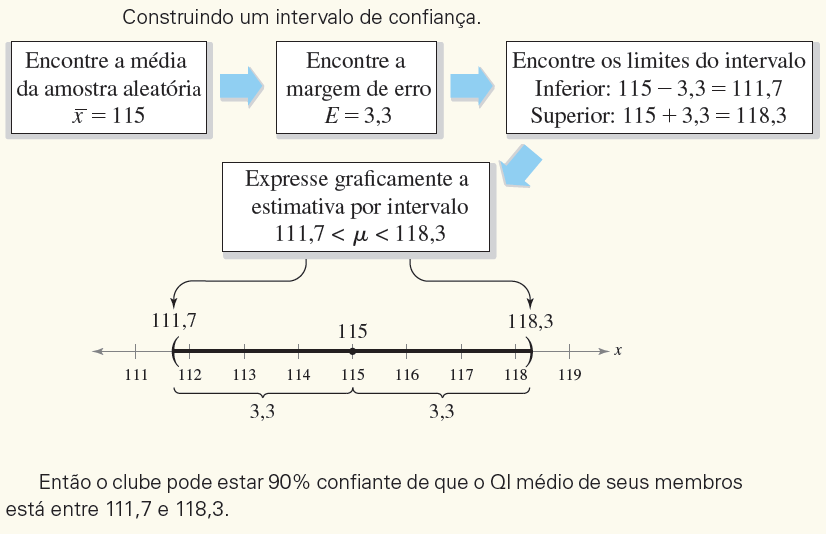
\includegraphics[scale=0.67]{figs/IC1.png}
\end{figure}
    \end{block}
\end{frame}

\begin{frame}{}

Logo, existem dois tipos de estimativas que podemos obter a partir de uma amostra aleatória:
\begin{block}{Estimativa Pontual}
\justifying
Fornecem como estimativa um único valor numérico para o parâmetro de interesse  
\end{block}

\begin{block}{Estimativa Intervalar}
\justifying
Fornece um intervalo de valores ``plausíveis'' para o parâmetro de interesse    
\end{block}
\end{frame}

\begin{frame}{}
    \begin{block}{}
    \justifying
Por serem \textbf{variáveis aleatórias}, os estimadores pontuais possuem uma distribuição de probabilidade (distribuições amostrais). Com isso, podemos apresentar uma estimativa mais informativa para o parâmetro de interesse, que inclua uma medida de precisão do
valor obtido, estimativa intervalar ou intervalo de confiança. Os \textbf{intervalos de confiança} são obtidos a partir da distribuição amostral de seus estimadores.    
\end{block}
\end{frame}

\section{Intervalos de Confiança para a Média: $\sigma$ conhecido}
\begin{frame}{}
    \begin{block}{Suposições necessárias}
    \justifying
\begin{itemize}
    \item A amostra é uma \textbf{amostra aleatória simples}. (Todas as amostras de mesmo tamanho tem a mesma probabilidade de serem selecionadas);\pause
    \item O valor do desvio padrão populacional $\sigma$, é conhecido; \pause
    \item Uma ou ambas das seguintes condições são satisfeitas:
    \begin{itemize}
        \item A população é normalmente distribuída;
        \item A amostra possui $n > 30$
    \end{itemize}
\end{itemize}
    \end{block}
\end{frame}

\begin{frame}{Erro Amostral}
    \begin{block}{}
    \justifying
    Quando coletamos uma \textbf{amostra aleatória} e calculamos uma média, sabemos que o valor da média possui um desvio natural, em relação ao verdadeiro valor da média populacional (\textbf{erro amostral}), ou seja
$$
e = \bar{X} - \mu \quad \Rightarrow \quad \bar{X} = \mu + e
$$

Sabemos que a \textbf{distribuição amostral da média} é uma distribuição normal, com média $\mu$ e variância
$\sigma^2/n$,
$$
\bar{X} \sim \text{N}\left(\mu, \frac{\sigma^2}{n}\right)
$$

    \end{block}
\end{frame}

\begin{frame}{Margem de Erro}
    \begin{block}{}
    \justifying
    Usando a transformação
$$
Z = \frac{\bar{X} - \mu}{\sigma/\sqrt{n}} =
\frac{e}{\sigma/\sqrt{n}} \, \sim \, \text{N}(0,1)
$$

podemos determinar o \textbf{erro máximo provável} que
assumimos para a média amostral que estamos calculando.
O \textbf{erro máximo provável} ou \textbf{margem de erro} da média é definido por
$$
e = z_{\gamma/2} \cdot \frac{\sigma}{\sqrt{n}}
$$

onde $z_{\gamma/2}$ é chamado de \textbf{valor crítico}.
    \end{block}
\end{frame}

\begin{frame}{Intervalo de Confiança}
\vspace{-0.3cm}
    \begin{block}{}
    \justifying
Fixando um valor $\gamma$ tal que $0 < \gamma < 1$, podemos encontrar um valor $z_{\gamma/2}$ tal que:
\vspace{-0.3cm}
\begin{align*}
&P(-z_{\gamma/2} < Z < z_{\gamma/2}) &= \gamma \\
\\
&P\Big(-z_{\gamma/2} < \frac{\bar{x} - \mu}{\sigma/\sqrt{n}} <
z_{\gamma/2}\Big) &= \gamma \\
\\
&P\Big(\bar{x} - z_{\gamma/2} \cdot
\left(\frac{\sigma}{\sqrt{n}} \right) < \mu < \bar{x} + z_{\gamma/2}
\cdot \left(\frac{\sigma}{\sqrt{n}} \right)\Big) &= \gamma \\
\\
&P(\bar{x} - e < \mu < \bar{x} + e) &= \gamma 
\end{align*}
    \end{block}
\end{frame}

\begin{frame}{}
    \begin{block}{}
    \justifying
O valor crítico $z_{\gamma/2}$ é o valor de $\gamma$ dividido por 2, uma vez que a ``massa'' $\gamma$ deve ser distribuída igualmente em torno de 0.    
    \end{block}
    
\begin{figure}
    \centering
    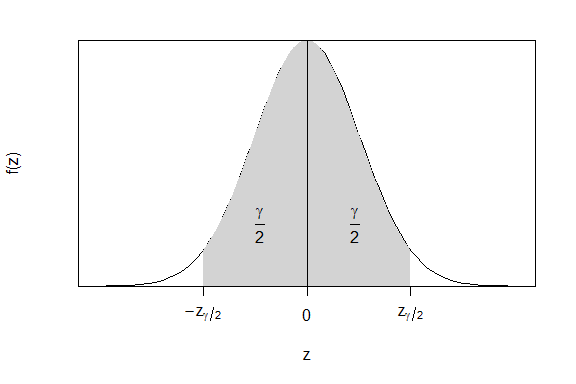
\includegraphics[scale=0.8]{figs/IC2.png}
\end{figure}
\end{frame}

\begin{frame}{}
    \begin{block}{}
    \justifying
A área $\gamma$ determina o \textbf{coeficiente de confiança} associado ao intervalo de confiança que estamos construindo. O valor $z_{\gamma/2}$ pode ser obtido da tabela da Normal padrão, localizando o valor de $\gamma/2$ no corpo da tabela e obtendo o valor $z_{\gamma/2}$ nas margens correspondentes. 
\begin{itemize}
    \item Exemplo: $\gamma = 0,95$:
    \begin{itemize}
    \item Temos que $\gamma/2 = 0,475$ é a área que devemos procurar no corpo da tabela

    \item O valor de $z_{\gamma/2}$ será determinado pelos valores correspondentes nas margens da tabela. Nesse caso, $z_{\gamma/2} = 1,96$ é o valor crítico procurado.   
\end{itemize}
\end{itemize}

    \end{block}
\end{frame}

\begin{frame}{}
    \begin{block}{}
    \justifying
Com estas definições, podemos construir um \textbf{intervalo de confiança} para $\mu$, com coeficiente de confiança $\gamma$:
$$
\text{IC}(\mu, \gamma) = \left[ \bar{X} - z_{\gamma/2} \cdot
  \left(\frac{\sigma}{\sqrt{n}}\right) ; \bar{X} + z_{\gamma/2} \cdot
  \left(\frac{\sigma}{\sqrt{n}}\right)  \right]
$$   
    \end{block}
\end{frame}

\begin{frame}{Procedimentos para a construção de intervalos de confiança}
    \begin{block}{}
    \justifying
\begin{enumerate}
    \item Verifique se as suposições necessárias estão satisfeitas
    \begin{itemize}
        \item Temos uma AAS
        \item $\sigma$ é conhecido
        \item A população tem distribuição normal ou $n>30$
    \end{itemize}
   
    \item Determine o nível de confiança $\gamma$, e encontre o valor crítico $z_{\gamma/2}$
    \item Calcule a margem de erro $e = z_{\gamma/2} \cdot (\sigma/\sqrt{n})$
    \item Calcule $\text{IC}(\mu, \gamma)$
\end{enumerate}   
    \end{block}
\end{frame}

\begin{frame}{Interpretação de um intervalo de confiança}
    \begin{block}{}
    \justifying
Como o intervalo de confiança é calculado a partir de uma amostra aleatória, este intervalo \textbf{também é aleatório}!

Isso significa que para cada amostra aleatória que tivermos, um intervalo diferente será calculado.

Como o valor de $\mu$ é fixo, é o intervalo que deve conter o valor de $\mu$, e não o contrário.

Isso significa que se pudéssemos obter 100 amostras diferentes, e calcularmos um intervalo de confiança de 95\% para cada uma das 100 amostras, esperaríamos que 5 destes intervalos \textbf{não} contenham o verdadeiro valor da média populacional $\mu$.   
    \end{block}
\end{frame}

\begin{frame}{}
    \begin{block}{}
    \justifying
   \begin{figure}
       \centering
       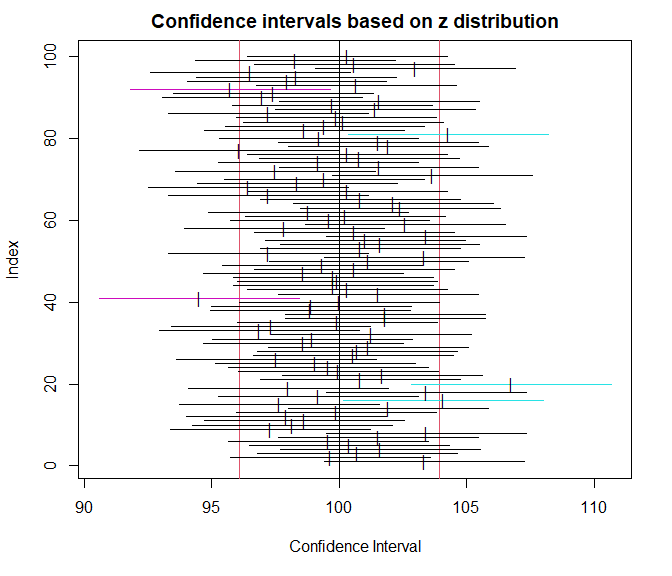
\includegraphics[scale=0.6]{figs/IC3.png}
   \end{figure}
    \end{block}
\end{frame}

\begin{frame}{Exemplo}
    \begin{block}{}
    \justifying
Uma empresa de computadores deseja estimar o tempo médio de horas semanais que as pessoas utilizam o computador. Uma amostra aleatória de 25 pessoas apresentou um tempo médio de uso de 22,4 horas. Com base em estudos anteriores, a empresa assume que $\sigma = 5,2$ horas, e que os tempos são normalmente distribuídos. Construa um intervalo de confiança para a média $\mu$ com coeficiente de confiança de 95%.   
    \end{block}
 \pause 
\begin{block}{}
%\begin{verbatim}
%xbar <- 22.4
%n <- 25
%sigma <- 5.2
%zcrit <- qnorm(.975)
%erro <- zcrit * sigma/sqrt(n)
%c(xbar - erro, xbar + erro)
$(20.36164\leq \mu\leq24.43836)$
%\end{verbatim}   
\end{block}
\end{frame}

\section{Intervalos de confiança para a média: $\sigma$ desconhecido}
\begin{frame}{Intervalos de confiança para a média: $\sigma$ desconhecido}
    \begin{block}{Estimativa da variância amostral}
    \justifying
Na maioria das situações práticas, não sabemos o verdadeiro valor do desvio padrão populacional $\sigma$. Se o desvio padrão é desconhecido, ele precisa ser estimado. Sendo $(X_1, \ldots, X_n)$ VAs onde $X \sim \text{N}(\mu, \sigma^2)$, vimos que o ``melhor'' estimador para $\sigma^2$ é a variância amostral
$$
S^2 = \frac{1}{n-1} (\sum_{i=1}^{n} X_i^2 - n\bar{X}^2)
$$   
que é não viciada e consistente para $\sigma^2$.   
\end{block}
\end{frame}

\begin{frame}{A distribuição $t$ de Student}
    \begin{block}{}
    \justifying
Definindo a variável padronizada
$$
T = \frac{\bar{X} - \mu}{\sqrt{S^2/n}} = \frac{\bar{X} - \mu}{S/\sqrt{n}}
$$   
o denominador $S^2$ fará com que a função densidade de $T$ seja diferente da Normal. Essa nova densidade é denominada \textbf{$t$ de Student}, e seu parâmetro é
denominado \textbf{graus de liberdade}, que nesse caso é $n-1$. Assim:
$$
T = \frac{\bar{X} - \mu}{S/\sqrt{n}} \, \sim \, t(n-1)
$$   
    \end{block}
\end{frame}

\begin{frame}{}
    \begin{block}{Valores Críticos de $t$}
    \justifying
Com a definição do \textbf{nível de confiança} e sabendo o tamanho da amostra $n$, sabemos então o valor de $\gamma$ e dos gl, e devemos encontrar o \textbf{valor crítico} de $t_{\gamma/2}$. Usando como exemplo $\gamma = 0,95$ e uma amostra de $n=7$

\begin{itemize}
    \item Temos que $n=7 \Rightarrow gl = n-1 = 6$

    \item Na tabela da distribuição $t$ de Student procure a linha correspondente aos gl, e  coluna correspondente ao valor de $1 - \gamma = 1 - 0,95 = 0,05 = 5\%$

    \item O valor de $t_{\gamma/2}$ será determinado pelos valores correspondentes \textbf{no corpo da tabela}. Nesse caso, $t_{\gamma/2} = 2,447$ é o valor crítico procurado.
\end{itemize}   
\end{block}
\end{frame}

\begin{frame}{}
    \begin{block}{}
    \justifying
 \begin{figure}
     \centering
     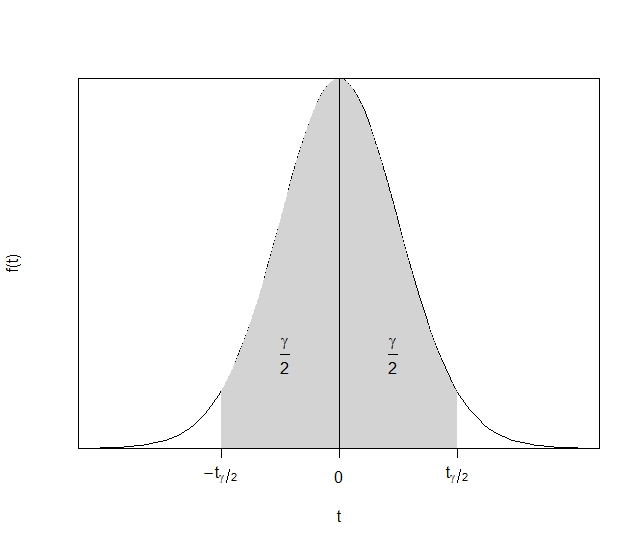
\includegraphics[scale=0.6]{figs/ICtStudent.jpeg}
 \end{figure}  
    \end{block}
\end{frame}

\begin{frame}{Intervalo de confiança}
    \begin{block}{}
    \justifying
Com estas definições, podemos construir um \textbf{intervalo de confiança} para $\mu$, com \textbf{coeficiente de confiança} $\gamma$, e
$\sigma$ desconhecido:
$$
\text{IC}(\mu, \gamma) = \left[ \bar{X} - t_{\gamma/2} \cdot
  \left(\frac{S}{\sqrt{n}}\right) ; \bar{X} + t_{\gamma/2} \cdot
  \left(\frac{S}{\sqrt{n}}\right)  \right]
$$   
   
    \end{block}
\end{frame}

\begin{frame}{Procedimentos para a construção de intervalos de confiança}
    \begin{block}{}
    \justifying
\begin{enumerate}
    \item Verifique se as suposições necessárias estão satisfeitas
    \begin{itemize}
        \item Temos uma AAS
        \item Temos uma estimativa de $s$
        \item A população tem distribuição normal ou $n>30$
    \end{itemize}
   
    \item Determine o nível de confiança $\gamma$, e encontre o valor crítico $t_{\gamma/2}$
    \item Calcule a margem de erro $e = t_{\gamma/2} \cdot (s/\sqrt{n})$
    \item Calcule $\text{IC}(\mu, \gamma)$
\end{enumerate}   
    \end{block}
\end{frame}

\begin{frame}{}
    \begin{block}{Exemplo}
    \justifying
Em um teste da eficácia do alho na dieta para a redução do colesterol, 51 pessoas foram avaliadas e seus níveis de colesterol foram medidos antes e depois do tratamento. As \textbf{mudanças} nos níveis de colesterol apresentaram média de 0,4 e desvio-padrão de
21. 
\begin{description}
\item[a)~]Para um nível de confiança de 95\%, calcule o intervalo para a verdadeira média das mudanças no nível de colesterol;
\item[b)~]O que o intervalo de confiança sugere sobre a eficácia do uso do alho na dieta para a redução do colesterol?
\item[c)~]Resolva o mesmo exemplo supondo que o $\sigma = s$ é conhecido (ou seja, usando a distribuição $Z$). Compare os dois métodos.
\end{description}
\end{block}
\end{frame}

\section{Intervalo de Confiança para Proporção}
\begin{frame}{Intervalo de Confiança para Proporção}
\vspace{-0.3cm}
\begin{block}{}
\justifying
A proporção amostral
$$
\hat{p} = \frac{x}{n} = \frac{\text{número de sucessos}}{\text{total de
tentativas}}
$$   
é a ``melhor estimativa'' para a proporção populacional $p.$ Através do estudo da distribuição amostral da proporção, chegamos aos seguintes resultados:

\begin{itemize}
    \item A proporção amostral $\hat{p}$ \textbf{tende} para o valor da proporção populacional $p$
    \item A distribuição das proporções amostrais tende a ser uma \textbf{distribuição normal}
    \item $\text{E}(\hat{p}) = \mu_{\hat{p}} = p$
    \item $\text{Var}(\hat{p}) = \sigma^{2}_{\hat{p}} = \frac{p(1-p)}{n}$
\end{itemize}
\end{block}
\end{frame}

\begin{frame}{Distribuição amostral da proporção $\hat{p}$}
    \begin{block}{}
    \justifying
Assim, sabemos que
$$
\hat{p} \sim \text{N} \left( p, \frac{p(1-p)}{n} \right)
$$   
É possível mostrar que a quantidade
$$
Z = \frac{\hat{p} - p}{\sqrt{\frac{p(1-p)}{n}}} \, \sim \, \text{N}(0,1)
$$   
    \end{block}
\end{frame}

\begin{frame}{}
    \begin{block}{Intervalo de Confiança}
    \justifying
  Logo, podemos construir um \textbf{intervalo de confiança} para $p$, com \textbf{coeficiente de confiança} $\gamma$
$$
\text{IC}(p, \gamma) = \left[ \hat{p} - z_{\gamma/2} \cdot
  \sqrt{\frac{p(1-p)}{n}} ;
  \hat{p} + z_{\gamma/2} \cdot
   \sqrt{\frac{p(1-p)}{n}}
  \right]
$$
\end{block}
\end{frame}

\begin{frame}{Procedimentos para a construção de intervalos de confiança}
    \begin{block}{}
    \justifying
\begin{enumerate}
    \item Verifique se as suposições necessárias estão satisfeitas
    \begin{itemize}
        \item Temos uma AAS
        \item As condições para a distribuição binomial são satisfeitas:
        \begin{itemize}
            \item as tentativas são independentes;
            \item há duas categorias de resultado (``sucesso'', ``fracasso'');
            \item a probabilidade de sucesso $p$ permanece constante;
        \end{itemize}
        \item A distribuição normal pode ser usada como aproximação para a    distribuição binomial, ou seja, $np \geq 5$ e $np(1-p) \geq 5$
    \end{itemize}
   
    \item Determine o nível de confiança $\gamma$, e encontre o valor crítico $z_{\gamma/2}$
    \item Calcule a margem de erro $e = z_{\gamma/2} \cdot \sqrt{\frac{p(1-p)}{n}}$
    \item Calcule $\text{IC}(\mu, \gamma)$
\end{enumerate}   
    \end{block}
\end{frame}

\begin{frame}{}
    \begin{block}{Exemplo}
    \justifying
Em uma pesquisa realizada por um instituto de pesquisa Norte-Americano, 1500 adultos foram selecionados aleatoriamente para responder à pergunta se acreditam ou não no aquecimento global. 1050 entrevistados responderam que sim. Com isso:

\begin{description}
\item[a)~]Para um nível de confiança de 95\%, calcule o intervalo de confiança para a verdadeira proporção de pessoas que acreditam no aquecimento global, utilizando:
 $(i)\ p = \hat{p} \text{ e } (ii)\ p = 0,5$ e compare os resultados.
\item[b)~]Com base nesses resultados, podemos concluir que a maioria dos adultos acredita no aquecimento global?
\end{description}   
\end{block}
\end{frame}

\section{Determinação do tamanho amostral ($\sigma$ conhecido)}
\begin{frame}{Determinação do tamanho amostral}
    \begin{block}{}
    \justifying
Nosso objetivo é coletar dados para estimar a \textbf{média populacional} $\mu$. A questão é:
\begin{center}
\textbf{Quantos elementos (itens, objetos, pessoas, ...) devemos amostrar?}   
\end{center}

Já vimos que, de maneira (bem) geral, $n>30$ é um tamanho de amostra mínimo para a maioria dos casos. Será que podemos ter uma estimativa melhor de quantos elementos devem ser amostrados para estimarmos a média populacional com uma precisão conhecida?   
\end{block}
\end{frame}

\begin{frame}{}
    \begin{block}{}
    \justifying
A partir da equação do \textbf{erro máximo provável}
$$
e = z_{\gamma/2} \cdot \frac{\sigma}{\sqrt{n}}
$$ 
podemos isolar $n$ e chegar na seguinte equação para a determinação do tamanho amostral
$$
n = \left[ \frac{z_{\gamma/2} \cdot \sigma}{e} \right]^2
$$
\end{block}
\end{frame}

\begin{frame}{}
    \begin{block}{}
    \justifying
Note que, em
$$
n = \left[ \frac{z_{\gamma/2} \cdot \sigma}{e} \right]^2
$$
\begin{itemize}
    \item O tamanho amostral $n$ \textbf{não} depende do tamanho populacional $N;$
    \item O tamanho amostral depende:
    \begin{itemize}
        \item do nível de confiança desejado (expresso pelo valor crítico $z_{\gamma/2}$);
        \item do erro máximo \textsl{desejado}
        \item do desvio-padrão $\sigma$ (embora veremos que não é estritamente necessário)
    \end{itemize}
    \item Como o tamanho amostral precisa ser um número inteiro, arredondamos sempre o valor para o \textbf{maior} número inteiro mais próximo.
\end{itemize}
\end{block}
\end{frame}

\begin{frame}{}
    \begin{block}{Exemplo}
    \justifying
Seja $X \sim \text{N}(\mu,36)$
\begin{description}
\item[a)~]Calcule o tamanho da amostra, para que com 95\% de probabilidade, a média amostral não difira da média populacional por mais de 
   \begin{itemize}
       \item $(i)\ 0,5 \text{ unidades} \quad (ii)\ 2 \text{ unidades}$
   \end{itemize}
\item[b)~]Qual o impacto do erro máximo assumido para o tamanho da amostra?
\item[c)~]Calcule o tamanho da amostra, para que a diferença da média amostral para a média populacional (em valor absoluto) seja menor ou igual a 2 unidades, com níveis de confiança de
\begin{itemize}
    \item $(i)\ 90\% \quad (ii)\ 95\%$
\end{itemize}
\item[d)~] Compare as estimativas do item anterior e analise o impacto do nível de confiança para a determinação do tamanho amostral.
\end{description}
\end{block}
\end{frame}

\section{Determinação do tamanho amostral ($\sigma$ desconhecido)}
\begin{frame}{Determinação do tamanho amostral ($\sigma$ desconhecido)}
    \begin{block}{}
    \justifying
Se $\sigma$ for desconhecido?
\begin{itemize}
    \item Estime o valor de $\sigma$ com base em algum estudo feito anteriormente
    \item Faça uma amostra piloto e estime o desvio padrão amostral $s$, e use-o como uma aproximação para o desvio-padrão populacional $\sigma$
    \item Use a \textbf{regra empírica} da amplitude para dados com distribuição (aproximadamente) normal
\end{itemize}
\end{block}
\end{frame}

\begin{frame}{Regra empírica para uma distribuição normal}
\begin{block}{}
\justifying
\begin{figure}
    \centering
    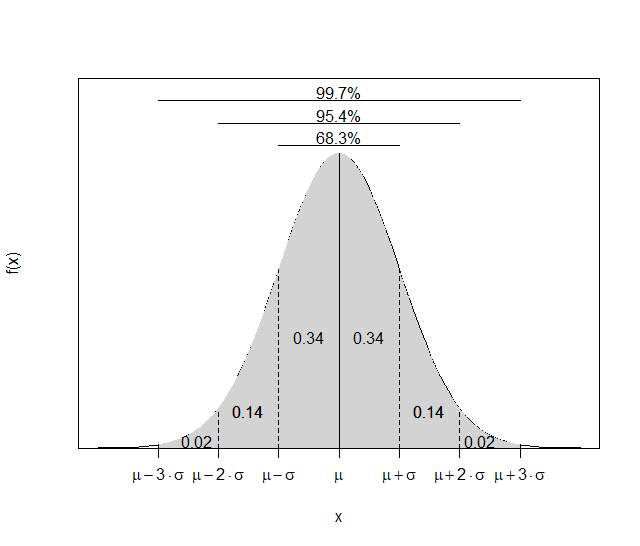
\includegraphics[scale=0.6]{figs/ICEmpirico.png}
\end{figure}
  
\end{block}
\end{frame}

\begin{frame}{Regra empírica para uma distribuição normal}
    \begin{block}{}
    \justifying
Define-se \textbf{valores usuais} aqueles que são típicos e não muito extremos. Como sabemos que em uma distribuição (aproximadamente) normal, aproximadamente 95\% dos dados encontram-se a 2 desvios-padrões acima e
abaixo da média, temos que
\begin{align*}
4\sigma &= (\max - \min) \\
\sigma &= \frac{(\max - \min)}{4}
\end{align*}
pode ser utilizado como uma estimativa para $\sigma$.  
\end{block}
\end{frame}

\begin{frame}{}
\begin{block}{Exemplo}
\justifying
Um professor deseja estimar o salário médio de professores do Ensino Médio de uma cidade. Quantos professores devem ser selecionados para termos 90\% de confiança que a média amostral esteja a menos de R\$30,00 da média populacional? Sabe-se apenas que os
salários variam entre R\$800,00 e R\$1.200,00. Use
$$
n = \left[ \frac{z_{\gamma/2} \cdot \sigma}{e} \right]^2
$$  
\nocite{Apostila}
%\begin{verbatim}
%zcrit <- qnorm(0.95)
%erro <- 30
%sigma <- (1200 - 800)/4
%((zcrit * sigma)/erro)^2    
%\end{verbatim}
\end{block}
\end{frame}

\begin{frame}%[allowframebreaks]
\frametitle{\bf Referências}
\printbibliography
\end{frame}


\end{document}
